\documentclass[journal]{IEEEtran}
% useful packages
\usepackage{
                graphicx, setspace, fontspec, caption,
                subcaption, float, polyglossia, rotating,
                lscape, pdflscape, indentfirst, tocloft,
                multirow, mathtools, currfile, xcolor, url,
                chngpage, slashbox
            }
\captionsetup{justification=centering}
% paragraph related package
\usepackage[parfill]{parskip}
% use bzar font(THIS MUST BE LOADED BEFORE XePerian PACKAGE)
\setmainfont{BZar.ttf}
% the dear XePersian package
\usepackage{xepersian}
%
% General settings goes here.
%
% lines space
\renewcommand{\baselinestretch}{1.5}
% paragraph first line indention
\setlength{\parindent}{1cm}
% paragraph spacing
\setlength{\parskip}{1em}
% set graphics' path
\graphicspath{ {images/} }
% make table of content dotted
\renewcommand{\cftsecleader}{\cftdotfill{\cftdotsep}}
% define a new command as {half-space} in english
\newcommand{\halfspace}{\hspace{0pt}}
% define a new command as {half-space} in persian
\newcommand{\نیمفاصله}{\halfspace}
% define a shortcut for half-space in general
\renewcommand{\ }{\halfspace}
% define a new command for ease of use for rendering reference
\newcommand{\renderref}[1] { \begingroup \let\clearpage\relax \include{#1} \endgroup }
% make IEEE sections' counter in arabic format
\def\thetable{\arabic{table}}
\def\thesection{\arabic{section}}
\def\thesubsection{\thesection.\arabic{subsection}}
\def\theparagraph{\thesubsubsection.\arabic{paragraph}}
\def\thesubsubsection{\thesubsection.\arabic{subsubsection}}

\newcommand{\وکا}{\lr{WEKA} }
\newcommand{\ار}{\lr{R} }
\renewcommand{\|}[1][.3em]{\hspace{#1}|\hspace{#1}}
\renewcommand{\,}[1][.3em]{,\hspace{#1}}

\newcommand*{\Scale}[2][4]{\scalebox{#1}{$#2$}}

\newcommand\Wider[2][3em]{%
\makebox[\linewidth][c]{%
  \begin{minipage}{\dimexpr\textwidth+#1\relax}
  \raggedright#2
  \end{minipage}%
  }%
}
%
% DOCUMENT BEGIN
%
\begin{document}
\title{شناسایی نشانه\ های حساب\ های جعلی با استفاده از تکنیک\ های داده\ کاوی}


\author{
\IEEEauthorblockN{محسن خالقی$^1$ و داریوش حسن\ پور آده$^2$}\\
\IEEEauthorblockA{
$^1$دانشگاه صنعتی اصفهان، دانشکده مهندسی برق و کامپیوتر\\
\lr{Email: {\tt mohesen.khaleghi@ec.iut.ac.ir}}\\}
\IEEEauthorblockA{
$^2$دانشگاه صنعتی اصفهان، دانشکده مهندسی برق و کامپیوتر\\
\lr{Email: {\tt d.hasanpoor@ec.iut.ac.ir}}}
}


%\date{}
\maketitle
\begin{abstract}
روش\ های شناسایی تقلب را می\ توان به دو دسته\ ی روش\ های تشخیص سوءاستفاده و تشخیص ناهنجاری تقسیم کرد. تکنیک\ های مبتنی بر رویکرد تشخیص سوء استفاده زمانی استفاده می\ شود که تشخیص تقلب به صورت از پیش\ شناخته شده بوده و بر اساس امضای تقلب می\ توان رفتار جاری مشتریان را بررسی نمود. طبیعتا به دلیل شناخت کامل رفتار قبلی مشتریان، دقت شناسایی تقلب در این روش بسیار بالاست. اما نقطه ضعف این روش\ ها، عدم پوشش\ دهی کامل محدوده\ ی تقلب می\ باشد. بدین معنی که فقط تقلب\ هایی شناسایی می\ شوند که حداقل یک بار رخ داده و یا امضای آن به سیستم تشخیص تقلب ارائه شده باشد. در مقابل این روش\ ها، روش های دیگری هم هستند که مبتنی بر تشخیص ناهنجاری اند. یعنی سعی می\ کنند رفتار آتی مشتری را پیش\ بینی کرده و به این منظور تاریخچه\ ی رفتار وی را مورد بررسی قرار می\ دهند. در این\ گونه روش\ ها، قاعده\ ی ثابت و مشخصی برای تعریف تقلب تعریف نمی\ شود بلکه رفتار عادی و نرمال مشتری به سیستم تشخیص تقلب آموخته شده و هرگونه انحراف از آن به معنی تقلب فرض می\ گردد. بدیهی است که دقت در این روش پایین\ تر ولی گستره\ ی تقلب های کشف شده بالاتر است. که در این کار بروی پیاده\ سازی روش اول تمرکز شده است.
\end{abstract}
\hspace{-.5cm}\
\textbf{کلمات\ کلیدی}\
\hspace{-.2cm}\begin{IEEEkeywords}
\textit{داده\ کاوی، تشخیص تقلب، بانکداری\ الکترونیکی}
\end{IEEEkeywords}

\IEEEpeerreviewmaketitle

\قسمت{مقدمه}
در تکنولوژی امروزی فرصت\ های بسیاری برای تقلب الکترونیکی به دلیل گسترش رسانه\ ها و شبکه\ های کامپیوتری وجود دارد. یکی از تقلب\ های معمول، تقلب در فرایند\ ها و تراکنش\ های خودپردازهای بانکی است. بدون توجه به نوع تقلبی که استفاده می\ شود، متقلبان تنها می\ توانند پول های قربانی را از حساب\ های متقلبانه جمع\ آوری کنند. بنابراین، شناسایی و کشف امضاهای این حساب\ های تقلبی بر اساس این
امضاها خیلی مهم است.\بند
روش شناسایی تقلب در این کار از تکنیک\ های مبتنی بر رویکرد تشخیص سوء استفاده زمانی می\ باشد، که تشخیص تقلب به صورت از پیش\ شناخته شده بوده که امضای تقلب می\ توان رفتار جاری مشتریان را مورد بررسی قرار می\ گیرد. طبیعتا به دلیل شناخت کامل رفتار قبلی مشتریان، دقت شناسایی تقلب در این روش بسیار بالاست. اما نقطه ضعف این روش\ ها، عدم پوشش\ دهی کامل محدوده\ ی تقلب می\ باشد. بدین معنی که فقط تقلب\ هایی شناسایی می\ شوند که حداقل یک بار رخ داده و یا امضای آن به سیستم تشخیص تقلب ارائه شده باشد.\بند
این مطالعه، رده\ بندی و قواعد\ انجمنی را برای شناسایی علائم حساب\ های جعلی و الگوهای معاملات جعلی مورد استفاده قرار می\ دهد که این قوانین بر اساس علائم شناسایی شده از قبل برای طراحی یک سیستم نظارتی مورد استفاده قرار می\ گیرد. در حالت کلی این کار شامل بخش\ های اصلی زیر خواهد بود:\\
مشابه هر پروژه\ ی داده\ کاوی دیگر داشتن یک دیتاست مناسب شرط اصلی به پایان رساندن آن پروژه است، لذا جستجو برای یک دیتاست مناسب به عنوان اولین قدم منطقی به نظر می\ رسد، ولی متاسفانه به علت ماهیت پروژه و داده\ های مورد استفاده در آن تقریبا تمامی\ داده\ های مورد استفاده در مقاله\ های مرتبط با این زمینه در دسترس عموم قرار داده نشده\ اند؛ بنابرین برخلاف حساسیت مساله به علت کمبود مجموعه\ ی داده\ های واقعی، مدل\ های زیادی برای تشخیص تقلب توسعه داده نشده\ اند. ولی با این\ حال ما از مجموعه داده\ های تقلب کارت\ های اعتباری آلمان\
\cite{DATASET:GERMAN}
که تقریبا تنها دیتاست در دسترس برای پروژه می\ باشد. با این حال این دیتاست خالی از ایراد نمی\ باشد؛ از ایرادات این دیتاست می\ توان به عدم نسبت حساب\ های تقلبی به حساب\ های عادی ٪۳۰ می\ باشد که بسیار زیاد است و همچنین ساختار داده\ ای ضعیفی دارد که در قسمت
\ref{sec:EDA}
بیشتر توضیح داده\ خواهد شد و دلیل دیگری برای اینکه چرا لزوما این دیتاست ایده\ ال برای کارهای تشخیص حساب\ های جعلی نمی\ باشد به تعداد بسیار کم این دیتاست(۱۰۰۰ رکورد) می\ توان اشاره کرد. فایل این دیتاست با فرمت \lr{ARFF} می\ باشد که یکی از فرمت\ های پشتیبانی شده در نرم\ افزار \وکا می\ باشد که در قسمت
\ref{sec:INSTRUMENTS}
توضیح مختصری درباره\ ی این نرم\ افزار ارائه می\ شود.\بند
بعد از یافتن دیتاست طبق اصول یادگرفته شده در طول ترم به کاوش و ارزیابی اولیه در میان داده\ ها می\ پردازیم که بتوان یک دیدگاه کلی نسبت به داده\ ها موجود در دست بدست بیاید که در نتایج این کاوش در بخش
\ref{sec:EDA}
 آورده شده است. سپس مطابق الگوی ارائه شده در مقاله نشانه\ های حساب\ های جعلی بدست می\ آوریم و نشانه\ های بدست آمده را با نشانه\ های معرفی شده در مقاله مقایسه می\ کنیم. در انتها یک بهبودی بر روی مدل ارائه شده در مقاله برای معماری سیستم تشخیص\ دهنده حساب\ های جعلی ارائه می\ کنیم.
\قسمت{پیشینه\ ی تحقیق}
\lr{Ghosh et al.}
در سال 1994\
\cite{RELWORKS:P1994}
یک مدل شبکه\ عصبی\زیرنویس{\lr{Neural Network}} سه\ لایه پیش\ خور\زیرنویس{\lr{Feed-Forward}} را ارائه کرده اند. این مدل برای شناسایی الگوهای تقلب استفاده شده است. در لایه\ ی خروجی یک مقدار عددی به عنوان رتبه\ ی تراکنش\زیرنویس{\lr{Transaction Rank}} ایجاد می\ شود که اگر از یک مقدار آستانه\ ای پایین\ تر باشد آن تراکنش به عنوان تراکنش تقلبی تشخیص داده می\ شود.
\\
\lr{Dorronsoro et al.}
در سال 1997\
\cite{RELWORKS:P1997}
نبز از روش شبکه\ های عصبی برای تشخیص تقلب استفاده کرده\ اند. برای ساختن مدل شبکه\ عصبی از یک آنالیز تفکیک\ کننده غیرخطی\زیرنویس{\lr{Non-linear Discriminant Analysis}} استفاده می\ شود. از آنجا که حجم بالایی از تراکنش\ ها باید در یک زمان مشخص مورد پردازش قرار گیرند، از یک سیستم امتیاز دهی استفاده شده است که برای امتیازدهی تنها از تراکنش\ هایی استفاده می\ کند که در یک بازه کوچک زمانی قبل از تراکنش مورد نظر رخ داده\ اند. این روش نسبت به روشی\ هایی که از همه\ ی تراکنش\ های پروفایل یک دارنده\ ی کارت استفاده می\ کنند، بخش بسیار کوچکتری از داده\ ها را بررسی می\ کند و در نتیجه کارایی بالاتری دارد.
\\
\lr{Chan et al.}
در سال 1999\
\cite{RELWORKS:P1999}
 یک روش توزیع شده برای کشف تقلب بکار برده\ اند. در این روش یک دیتاست بزرگ با داده\ های برچسب\ دار به چند زیرمجموعه\ ی کوچکتر تقسیم می\ شوند. سپس تکنیک\ های داده\ کاوی روی هریک از این زیرمجموعه\ ها اعمال شده و یک طبقه\ کننده\زیرنویس{\lr{Classifier}} برای هر کدام از زیرمجموعه\ ها بدست می\ آید. سپس از یک روش \lr{Meta-Learning} استفاده می\ شود تا از ترکیب این طبقه\ کننده\ ها یک فرا-طبقه\ کننده ساخته می\ شود. در این روش هر یک از طبقه\ کننده\ ها به صورت یک جعبه سیاه دیده می\ شود. به این معنی که از هر الگوریتم یادگیری می\ توان در ایجاد آن\ ها استفاده نمود. در این تحقیق از 5 الگوریتم \lr{Bayes\, C4.5\, ID3\, CART\, Ripper} استفاده شده\ است. هم چنین در سیستم ارائه شده می\ توان از داده\ های توزیع شده نیز استفاده نمود، به این معنی که طبقه\ کننده\ هایی که از داده\ های مجزا و توزیع شده بدست آمده\ اند با هم ترکیب می\ شوند. اگر فرمت دیتاست\ ها با یکدیگر سازگار نباشد از یکی از دو روش برای سازگاری استفاده می\ شود؛ در روش اول یک عامل پل\ زنی در دیتاستی که شامل صفاتی اضافه بر دیتاست دیگر است ساخته می\ شود که وظیفه آن تخمین مقادیر این صفت در دیتاست فاقد این صفت است. سپس از روی این مقادیر تخمینی طبقه\ کننده دیتاست دوم ایجاد می\ شود. در روش دوم برای دیتاستی که شامل صفاتی اضافه بر دیتاست دیگر است دو طبقه\ کننده یکی فاقد صفت مزبور و دیگری با در نظر گرفتن صفت مزبور ساخته می\ شود. از طبقه\ کننده اول برای تبادل اطلاعات و از طبقه\ کننده دوم به صورت محلی استفاده می\ شود. هم چنین در این سیستم به دلیل اینکه طبقه\ کننده\ های زیادی ساخته می\ شود ممکن است برخی از آنها افزونه باشند. لذا از روش هایی برای هرس کردن طبقه\ کننده\ ها و ایجاد یک مجموعه بهینه از آنها استفاده می\ گردد. برای ترکیب طبقه\ کننده\ ها نیز از روش های متعددی می\ توان استفاده نمود. یک روش \lr{Class-Combiner} است که یک مجموعه\ ی آزمایشی می\ سازد که صفات آن پیش\ بینی\ های هر یک از دسته\ کننده\ هاست و برچسب آن نیز برچسب واقعی طبقه\ بندی است. سپس از این مجموعه\ ی آزمایشی برای یادگیری یک طبقه\ کننده\ ی ترکیبی استفاده می\ شود. این روش از روش\ های رای\ گیری مثل روش \lr{Adaboost} بسیار کاراتر عمل می\ کند. این سیستم به موسسات مالی امکان می\ دهد که مدل\ های تقلب خود را از طریق طبقه\ کننده\ ها با یکدیگر مبادله کنند.
\\
\lr{Tue et al.}
در سال 2004\
\cite{RELWORKS:P2004}
 چارچوبی بر پایه سیستم\ های ایمنی و
\lr{Case Based Reasoning}
برای تشخیص تقلب ارائه داده\ اند. ابتدا مجموعه\ ای از موارد نرمال و تقلبی از روی داده\ های برچسـب\ دار ساخته می\ شود. سپس کشف\ کننده\ های اولیه با الگوریتم\ های تصادفی و یا ژنتیک ساخته می\ شوند. سپس عملیات
\lr{Negative Selection} و \lr{Clonal Selection}
بر روی کشف\ کننده\ های اولیه اعمال می\ شود تا مجموعه\ ای از کشف\ کننده\ ها با الگوهای متفاوت بدست آید که می\ توانند انواع تقلب را کشف کنند. زمانی که یک تراکنش جدید می\ آید، شباهت این تراکنش با کشف\ کننده\ ها محاسبه می\ شود و اگر این شباهت از آستانه\ ای بالاتر بود هشدار داده می\ شود. پس از تایید یک فرد خبره مبنی بر تقلبی بودن یا نبودن آن تراکنش، از آن برای بهبود مـدل استفاده می\ شود.
\\
\lr{Vatsa et al.}
در سال 2005\
\cite{RELWORKS:P2005}
 یک سیستم دو لایه ارائه داده\ اند که در لایه\ ی اول قوانین عمومی\ و قوانین خاص هر مشتری بکار گرفته می\ شود تا درجه\ ی مشکوک بودن یک تراکنش را مشخص کند. اما از آنجا که این قوانین ثابت هستند و ممکن است میزان تراکنش\ های تقلبی که تشخیص داده نمی\ شوند و تراکنش\ های غیرتقلبی که به عنوان تقلبی معرفی می\ شوند زیاد باشد لایه دومی\ به کار گرفته می\ شود که از تکنیک\ های تئوری\ بازی برای تشخیص تقلب استفاده می\ کند. فرد متقلب و سیستم تشخیص تقلب دو طرف این بازی هستند که هریک سعی دارند سود خود را ماکزیمم کنند.
\\
\lr{Gadi et al.}
در سال 2008\
\cite{RELWORKS:P2008}
 از ۵ روش دسته\ بندی برای تشخیص تقلب استفاده کرده\ اند:
\lr{Neural Network\, Naive Bayes\, Bayesian Network\, Artificial Immune System} و \lr{Decision Tree.}
برای پیاده\ سازی این روش\ ها از ابزار \وکا استفاده شده\ است. به جز روش
\lr{Artificial Immune System}
 که برنامه جداگانه\ ای برای آن نوشته شده\ است، هریک از این روش\ ها در دو حالت حساس به هزینه و سـاده ارزیابی شده\ اند. به\ این معنی که در حالت اول هزینه\ ی مربوط به موارد نرمالی که به اشتباه تقلبی تشخیص داده می\ شوند با هزینه\ ی مربوط به موارد تقلبی که به اشتباه نرمال تشخیص داده می\ شوند متفاوت است. هم چنین برای روش\ هایی که پارامتری هستند یکبار با پارامترهای پیش فرض \وکا و یکبار با پارامترهای بهینه شده مورد ارزیابی قرار گرفته\ اند. نتایج مقایسه\ ی این دو حالت نشان می\ دهد که در هیچ یک از روش\ ها پارامترهای پیش فرض \وکا بهینه نبوده\ اند. برای بهینه\ سازی پارامترها از الگوریتم ژنتیک استفاده شده\ است.

\قسمت{ابزارهای مورد استفاده}
\label{sec:INSTRUMENTS}
برای به نهایت رساندن پروژه در کنار از نرم\ افزار \وکا که به خاطر راحتی برای مراحل تجزیه و تحلیل اکتشافی داده\ ها\زیرنویس{\lr{Exploratory Data Analysis (EDA)}}؛ از زبان برنامه\ نویسی \ار برای مراحل مدل\ سازی استفاده می\ کنیم. که در زیر توضیحی خلاصه\ ای در مورد هریک از ابزارهای فوق\ الذکر ارائه می\ دهیم.
\زیرقسمت{نرم\ افزار \وکا}
وکا نام یک نرم‌افزار متن‌\ باز\زیرنویس{\lr{Open Source}}  است که شامل مجموعه‌ای از الگوریتم\ های یادگیری ماشینی و داده\ کاوی می\ شود. این ابزار در دانشگاه وایکاتو در کشور نیوزلند توسعه داده شده است. وکا در تحلیل داده\ های عظیم کاربرد دارد. تمام قسمت\ های این نرم\ افزار به زبان\ جاوا نوشته شده\ است و در نتیجه می\ تواند بر روی هر پلتفرمی\زیرنویس{\lr{Platform}} اجرا گردد. رابط اصلی کاربری \وکا اکسپلورر\زیرنویس{\lr{Explorer}} است، اما با استفاده از خط فرمان نیز امکانات اکسپلورر قابل دسترسی است. همچنین آزمونگر\زیرنویس{\lr{Experimenter}} نیز امکان اجرای الگوریتم‌های مختلف رده\ بندی به صورت هم\ زمان و مقایسه نتایج آن\ ها وجود دارد. تمامی شاخص\ های مورد نیاز به منظور بررسی مدل\ های رده\ بندی در این قسمت تعریف شده و قرار دارند و گزارشات مفصلی را از جمله آزمون $T$ می توان در این قسمت پس از مدلسازی استخراج نمود.

\زیرقسمت{زبان برنامه\ نویسی \ار}
\ار یک زبان برنامه‌نویسی و محیط نرم‌افزاری متن\ باز برای محاسبات آماری و تحلیل داده است، که بر اساس زبان\ های \lr{S} و \lr{Scheme} پیاده\ سازی شده است. از ویژگی\ های \ار می\ توان گفت که \ار، حاوی محدوده\ ی گسترده\ ای از تکنیک\ های آماری (از جمله: مدل‌سازی خطی و غیرخطی، آزمون‌های کلاسیک آماری، تحلیل سری‌های زمانی، رده‌بندی، خوشه‌بندی و غیره) و قابلیت\ های گرافیکی است. در محیط \ار، کدهای \lr{C, C++, Fortran} قابلیت اتصال و فراخوانی هنگام اجرای برنامه را دارند.

\قسمت{تجزیه و تحلیل اکتشافی دیتاست}
\label{sec:EDA}
در این قسمت به بررسی دیتاست انتخاب شده می\ پردازیم؛ در جواب این سوال که آیا این دیتاست متشکل از داده\ های واقعی می\ باشد یا خیر با توجه به تعداد کم داده\ ها با تردید می\ توان سخن گفت. بعد از آنکه دیتاست را در قسمت اکسپلورر نرم\ افزار \وکا بارگذاری کردیم گزاش اولیه\ ای از وضعیت دیتاست بدست می\ دهد این است که این دیتاست شامل ۱۰۰۰ رکورد است و هر رکورد از ۲۱ ویژگی متشکل شده است که در هیچ از رکوردها ویژگی\ ای  گم نشده است. جدول
\ref{tbl:EDA:attribs}
مشخصات این ویژگی\ ها آورده شده است.\بند
\begin{table*}[ht]
\centering
\begin{latin}
\begin{adjustwidth}{-.34in}{0in}
\begin{tabular}{l|l|c|l}
Attributes & Description & Data Type & Valid Ranges/Categories\\\hline
over\_draft & Status of existing checking account & Qualitative & $\{<0\, 0\leq\ldots<200\, \geq20\,\text{no checking}\}$\\
credit\_usage & Duration in month & Numerical & \textbf{--} \\
credit\_history & Credit history & Qualitative & \footnotesize{'no credits/all paid'\, 'all paid'\, 'existing paid'\, \ldots}\\
purpose & Purpose & Qualitative & \footnotesize{'new car'\, 'used car'\, 'furniture/equipment'\, \ldots}\\
current\_balance & Credit amount & Numerical & \textbf{--} \\
Average\_Credit\_Balance & Savings account/bonds & Qualitative & \scriptsize{$\{<100\, 100\leq\ldots<500\, 500\leq\ldots<1000\,\ldots\}$}\\
employment & Present employment since & Qualitative & \scriptsize{$\{\text{unemployed}\, <1\, 1\leq\ldots<4\, 4\leq\ldots<7\, \geq7\}$}\\
location & Installment rate in percentage of disposable income & Numerical & \textbf{--} \\
personal\_status & Personal status and sex & Qualitative & \footnotesize{'male div/sep'\, 'female div/dep/mar'\, 'male single'\, \dots}\\
other\_parties & Other debtors / guarantors &  Qualitative & \footnotesize{'none'\, 'co applicant'\, 'guarantor'}\\
residence\_since & Present residence since & Numerical & \textbf{--} \\
property\_magnitude & Property & Qualitative & \footnotesize{'real estate'\, 'life insurance'\, 'car'\, 'no known property'}\\
cc\_age & cc\_age in months & Numerical & \textbf{--} \\
other\_payment\_plans & Other installment plans & Qualitative & \footnotesize{'bank'\, 'stores'\, 'none'}\\
housing & Housing & Qualitative & \footnotesize{'rent'\, 'own'\, 'for free'}\\
existing\_credits & Number of existing credits at this bank & Numerical & \textbf{--} \\
job & Job & Qualitative & \footnotesize{'unemp/unskilled non res'\, 'unskilled resident'\, \ldots}\\
num\_dependents & Number of people being liable to provide maintenance for & Numerical & \textbf{--} \\
own\_telephone & Telephone & Qualitative & \footnotesize{'yes'\, 'none'}\\
foreign\_worker & Foreign worker & Qualitative & \footnotesize{'yes'\, 'no'}\\
class & Fraud status & Qualitative & \footnotesize{'good'\, 'bad'}\\
\end{tabular}
\end{adjustwidth}
\end{latin}
\caption{جزئیات ویژگی\ های دیتاست\cite{DATASET:GERMAN}}\label{tbl:EDA:attribs}
\end{table*}

بعد از بارگذاری دیتاست در \وکا در تب\زیرنویس{\lr{Tab}}
\lr{Preprocess}
نرم افزار یک دید کلی نسبت به توزیع داده\ ای هریک از ویژگی\ ها و نسبت آنها به متغییر هدف که در اینجا ویژگی
\lr{Class}
می\ باشد، ارائه می\ دهد. که در اینجا کارت\ های اعتباری\ ای که به عنوان جعلی نشانه\ گذاری\زیرنویس{\lr{Flag}} شده\ اند با رنگ قرمز نشان داده شده\ اند. در این تب با انتخاب هر کدام از ویژگی\ ها می\ توان توزیع داده\ ای آن متغییر نسبت به متغییر هدف و همچنین توزیع آماری داده\ های آن متغییر در کل دیتاست را مشاهده کرد(که برای متغییرهای دسته\ ای تعداد رکوردهای مرتبط با هر کدام از دسته\ ها را می\ آورد و برای متغییر عددی مقادیر حداقل و حداکثر و میانگین و انحراف از معیار را ارائه می\ دهد.)، که یک نمونه در شکل
\ref{fig:EDA:weka-preprocess-dist}
آورده شده است.\بند
\begin{figure}
\centering
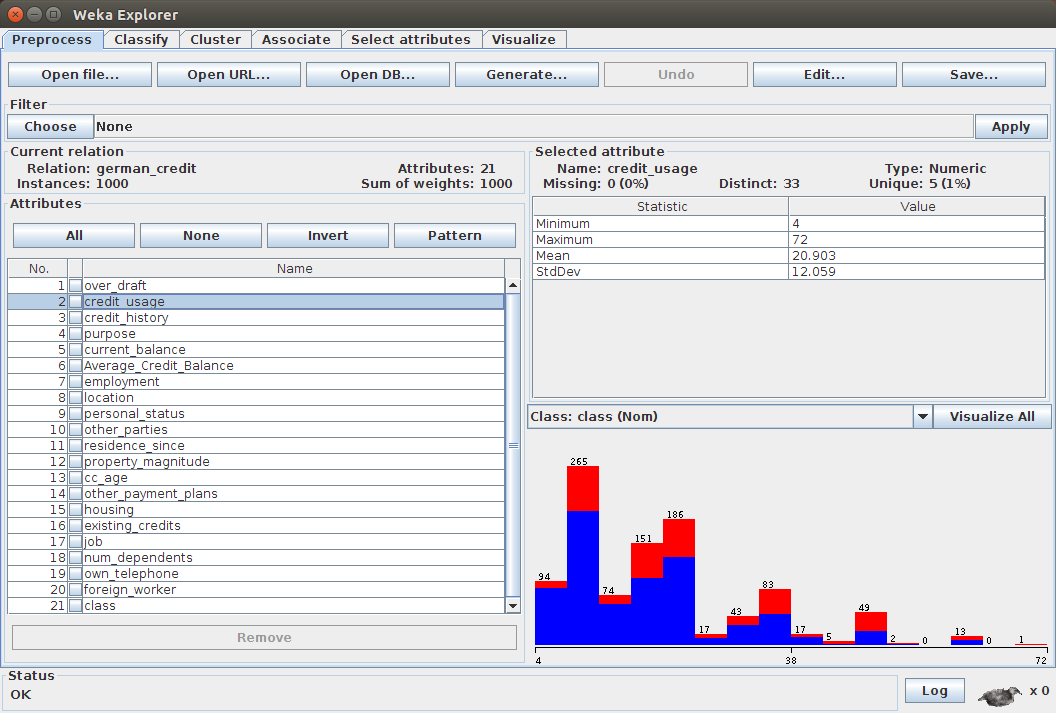
\includegraphics[width=.5\textwidth]{weka-preprocess-dist}
\caption{نمونه مثال نمایش توزیع داده\ ای در \وکا مرتبط با متغییر \lr{credit\_usage}}\label{fig:EDA:weka-preprocess-dist}
\end{figure}
همچنین در تب
\lr{Visualize}
که مختص به تصویر کردن داده\ ها می\ باشد، توزیع هر دو متغییر را نسبت به هم ارائه می\ دهد. با انتخاب بر روی یکی از نمودارها یک پنجره\ ی دیگر باز می\ شود که متغییرها را براساس یک\ دیگر نمایش داده است؛ از این پنجره اگر بروی هریک از نمودارهای موجود در سمت راست پنجره انتخاب کنیم متغییر روی محور افقی نمودار را عوض میکنیم. اگر در تب
\lr{Visualize}
بروی یکی از نمودارهای سطر اول کلیک کنیم از پنجره\ ای که باز می\ شود، می\ توانیم توزیع متغییر هدف را بر اساس تک\ تک متغییر\ ها مشاهده کنیم، که در این نمودارها محور افقی متغییر مستقل دیتاست و محور عمودی متغییر وابسته(هدف) می\ باشد. که بعد از گشتی در میان این نمودارها به راحتی می\ توان نتیجه گرفت که هیچ یک از متغییرها \textbf{به تنهایی} ضریب همبستگی بالایی با متغییر هدف ندارند(به علت عدم مشاهده\ ی عینی الگویی میان متغییر مستقل و متغییر وابسته)، لذا برای اینکه بتوان مدلی ارائه داد نیاز داریم متغییرهای توامی را انتخاب کنیم که دارای ضریب همبستگی بالایی با متغییر هدف دارند، که انتخاب اینکه کدامین متغییرها مدل بهتری برای پیشبینی و توصیف متغییر هدف را می\ تواند ارائه دهد را با استفاده از الگوریتم\ های داده\ کاوی که بخش
\ref{sec:MODEL_EXTARCTION}
آورده شده است.\\
\قسمت{استخراج مدل}
\label{sec:MODEL_EXTARCTION}
ما تصمیم گرفتیم که متغییر پیش\ بین را با استفاده از ۳ الگوریتم بیزین\ ساده\زیرنویس{\lr{Naïve Bayesian}}،
\lr{SVM}
و درخت\ تصمیم پیش\ بینی کنیم، ما بعد از بارگذاری دیتاست، آن را به میزان ۱۰۰ بار بر زدیم\زیرنویس{\lr{Shuffle}} که احتمال اینکه یک توزیع متناسب و یکسان برای هریک از مجموعه داده\ های آموزشی و تست بالا باشد. سپس ما داده\ ی آموزشی را به نسبت ۷ به ۱۰ به دو مجوعه آموزشی و تست تقسیم می\ کنیم و سپس این مجموعه\ ها را در دو فایل ذخیره می\ کنیم که از دفعات بعدی فقط آن\ ها بارگذاری کنیم و از تقسیم مکرر و غیر ضروری داده\ ی آموزشی و تقسیم بعدی آن اجتناب کنیم.\بند
بعد از این\ که داده\ های آموزشی و تست بارگذاری شدند، داده\ ی آموزشی را به هریک از ۳ الگوریتم\ های یادگیری مدل اشاره شده داده می\ شود و مدل استخراج شده هریک را در یک متغییر ذخیره می\ کنیم، سپس داده\ های تست را به مدل\ های استخراج شده می\ دهیم و نتایج را در قابل یک ماتریس درهم\ ریختگی\زیرنویس{\lr{Confusion Matrix}} نمایش می\ دهیم. نتایج حاصل از این مدل\ ها در جدول
\ref{tab:PRIOR_RESULTS}
آمده\ است.

\begin{table}[ht]\small
\centering
\def\arraystretch{1.5}
\begin{latin}
\begin{tabular}{l|c|c|c}
Measures & Naive Bayesian & SVM & Decision Tree\\\hline
Accuracy & 0.76 & 0.77 & 0.72\\
95\% CI & (0.70, 0.80) & (0.71, 0.81) & (0.66, 0.77)\\
Sensitivity & 0.53 & 0.36 & 0.45\\
Specificity & 0.85 & 0.94 & 0.84\\
P-Value & 0.013 & 0.003 & 0.173
\end{tabular}
\end{latin}
\caption{نتایج هریک از مدل\ های استخراج شده توسط ۳ الگوریتم بیزین\ ساده،
\lr{SVM}
  و درخت تصمیم برای داده\ های تست}
\label{tab:PRIOR_RESULTS}
\end{table}

همان\ طور که می\ بینیم الگوریتم \lr{SVM} مدل بهتری را برای پیش\ بینی متغییر هدف ارائه داده\ است ولی در اینجا سوالی مطرح می\ شود که چگونه می\ توان سیستم جامعی طراحی کرد که بتواند این مدل\ ها را باهم به کار گیرد؟ زیرا که لزوما برای یک نمونه هر ۳تای این مدل\ ها یک پیش\ بینی یکسانی را ارائه نمی\ دهند، مثلا برای یک نمونه احتمال این\ که آن نمونه به کدام یک از کلاس\ ها می\ باشد در جدول
\ref{tab:PROB_SAMPLE_PRED}
آمده است\زیرنویس{این نمونه و احتمالات یک مثال واقعی از مجموعه\ داده\ ی تست می\ باشد.}.

\begin{table}[ht]\small
\centering
\def\arraystretch{1.5}
\begin{latin}
\begin{tabular}{c|c|c}
\backslashbox{Algorithm}{Class} & Bad & Good \\\hline
Naive Bayesian & 0.165 & 0.835 \\
SVM & 0.502 & 0.498 \\
Decision Tree & 0.192 & 0.808
\end{tabular}
\end{latin}
\caption{احتمالات تعلق به کلاس\ ها برای یک نمونه از مجموعه داده\ ی تست}
\label{tab:PROB_SAMPLE_PRED}
\end{table}

نمونه\ ای در جدول فوق که احتمالات تعلقش به کلاس\ ها آورده شده است در اصل به کلاس
\lr{Good}
متعلق است، همان\ طور که می\ بینیم دو مدل بیزین\ ساده و درخت\ تصمیم درست ارزیابی کرده\ اند ولی مدل \lr{SVM} در تصمیم\ گیری راجع به کلاس نمونه مردد است. با اینکه همان\ طور که در جدول
\ref{tab:PRIOR_RESULTS}
آمده است، \lr{SVM} مدل بهتری نسبت به دیگر الگوریتم\ ها ارائه داده است ولی در اینجا دیگر مدل\ ها بهتر توانسته\ اند دسته\ بندی کنند.\بند
حال با برگشت به سوالی که قبلا مطرح کرده بودیم میبنی بر اینکه «چگونه می\ توان سیستم جامعی طراحی کرد که بتواند این مدل\ ها را باهم به کار گیرد؟» ما انتگرال فازی چوکت\زیرنویس{\lr{Fuzzy Choquet Integral}} را برای این منظور معرفی می\ کنیم.
\زیرقسمت{انتگرال فازی چوکت}
توضیح دقیق راجع به انتگرال فازی چوکت از حوصله\ ی موضوع این نوشتار خارج است ولی بطور خلاصه اگر بخواهیم هدف این انتگرال را معرفی کنیم، می\ توان گفت که این انتگرال برای ترکیب اطلاعات منابع که دارای خاصیت اندازه\ گیری-غیرافزایشی\زیرنویس{\lr{Non-Additive Measure}} می\ باشد؛ معرفی شده است. خاصیت اندازه\ گیری-غیرافزایشی در حالت کلی می\ گوید که اهمیت بودن چند منبع اطلاعاتی با هم برابر با مجموع اهمیت تک\ تک آن\ ها نمی\ باشد. به عنوان مثال:
\[\mu(\{1\,2\}) \neq \mu(\{1\}) + \mu(\{2\})\]
انتگرال فازی چوکت را به صورت
\ref{eq:CHOQUET_INTEGRAL}
معرفی می\ کنیم.
\begin{align}
    &\mathcal{C}_\mu(x) = \sum_{i = 1}^n (x_{\tau(i)} - x_{\tau(i - 1)})\mu(\{\tau(i),\ldots,\tau(n)\})\label{eq:CHOQUET_INTEGRAL}\\
    &\Scale[0.8]{x_{\tau(1)}{\leq}x_{\tau(2)}\leq\ldots{\leq}x_{\tau(n)}}\,\Scale[0.8]{x_{\tau(0)} = 0}\nonumber
\end{align}
که در آن $n$ تعداد مدل\ های بدست آمده است(که در مورد کار ما
$n = 3$
می\ باشد.) و $x_i$ میزان احتمال تعلق نمونه به کلاس \lr{Good} می\ باشد و مجموعه\ ی $\tau$ اندیس مدل\ های مرتب شده با توجه به میزان احتمال تعلق به کلاس \lr{Good} می\ باشد. $\mu$ نیز میزان اهمیت نتایج ترکیب الگوریتم\ ها با هم می\ باشد که بطور تجربی و با استفاده از دید کلی\ ای که  از عملکرد ۳ الگوریتم داریم تنظیم کرده\ ایم که به صورت زیر می\ باشند.
\vspace{-2em}\begin{latin}
\begin{align*}
	&\mu(\{\emptyset\}) = 0\,\mu(\{\text{NB}\,\text{SVM}\,\text{TR}\}) = 1\\
	&\mu(\{\text{NB}\}) = \mu(\{\text{SVM}\}) = \mu(\{\text{TR}\}) = {1 \over 3}\\
	&\mu(\{\text{NB}\,\text{SVM}\}) = 0.8\\
	&\mu(\{\text{NB}\,\text{TR}\}) = \mu(\{\text{SVM}\,\text{TR}\}) = {2 \over 3}
\end{align*}
\end{latin}
همان\ طور که می\ بینیم خواصیت اندازه\ گیری-غیرافزایشی در درجات اهمیت فوق مشاهده می\ شود.
\زیرقسمت{استخراج مدل نهایی با استفاده از انتگرال فازی چوکت}
با درنظر گرفتن انتگرال چوکت می\ توان به مدل\ های بدست آمده قبلی به عنوان مدل\ های میانی نگاه کرد و مدل نهایی که از ترکیب مدل\ های آن\ ها با استفاده از انتگرال چوکت بدست می\ آید به عنوان مدل نهایی در نظر گرفت. که نتایج مدل\ هایی بدست آمده برای طبقه\ بندی نمونه\ های تست مورد استفاده در جدول
\ref{tab:PRIOR_RESULTS}
به صورت
\ref{tab:FINAL_RESULTS}
آمده است.
\begin{table*}[ht]\scriptsize
\centering
\def\arraystretch{1.5}
\begin{latin}
\begin{tabular}{l|c|c|c|c}
Measures & Naive Bayesian & SVM(kernel $\rightarrow$ rbfdot) & Decision Tree & \textbf{FCI}\\\hline
Accuracy & 0.76 & 0.77 & 0.72 & \textbf{0.78}\\
95\% CI & (0.70, 0.80) & (0.71, 0.81) & (0.66, 0.77) & \textbf{(0.73, 0.83)}\\
Sensitivity & 0.53 & 0.36 & 0.45 & \textbf{0.52}\\
Specificity & 0.85 & 0.94 & 0.84 & \textbf{0.90}\\
P-Value & 0.013 & 0.003 & 0.173 & \textbf{0.0003}
\end{tabular}
\end{latin}
\caption{مقایسه\ ی نتایج بدست آمده با مدل نهایی با استفاده از انتگرال چوکت با نتایج قبلی}
\label{tab:FINAL_RESULTS}
\end{table*}
همان\ طور که می\ بینیم در حالت کلی مدل ارائه شده توسط انتگرال چوکت از مدل\ های تکی بهتر عمل کرده است.
\قسمت{نتایج بدست آمده با استفاده از دیگر الگوریتم\ های طبقه\ بند}
مدل ارائه و کد شده\ ای که در قسمت
\ref{sec:MODEL_EXTARCTION}
ارائه شد، سعی شده بود علاوه بر کدنویسی و ارائه این ایده که از انتگرال فازی می\ توان برای ایجاد یک مدل که در صورت نتظیم صحیح و معقولانه\ ی پارامترهای این انتگرل می\ تواند لزوما یک مدل بهتری نسبت به دیگر مدل\ ها ارائه دهد، در این قسمت نتایج الگوریتم\ های متنوع\ ای که با استفاده از جعبه\ ابزار ارائه شده توسط \وکا بدست آمده است را در جدول
\ref{tab:OTHER_RESULTS}
آورده\ ایم. در تمامی این الگوریتم\ ها از روش تست
\mbox{\lr{10-FOLD}}
استفاده شده است.
\begin{table}[ht]\small
\centering
\def\arraystretch{1.5}
\begin{latin}
\begin{tabular}{l|c|c}
Algorithm & Accuracy & ROC \\\hline
Neural Network   & 0.720 & 0.733 \\
LOG & 0.752 & 0.785 \\
LOG Simple & 0.759 & 0.792\\
Bayas Net & 0.755 & 0.780\\
Meta. Classification via Regression & 0.759 & 0.780\\
Meta. Multiclass Classifier & 0.752 & 0.785\\
Meta. Random Committee & 0.739 & 0.785\\
Hoeffding Tree & 0.750 & 0.785\\
Tree. LMT & 0.759 & 0.792
\end{tabular}
\end{latin}
\caption{دقت\ ها و مساحت زیر سطح نمودار
\lr{ROC}
برای الگوریتم\ های متفاوت -- اجرا شده در \وکا
}
\label{tab:OTHER_RESULTS}
\end{table}
اگر نتایج نشان داده شده در جدول
\ref{tab:FINAL_RESULTS}
با جدول
\ref{tab:OTHER_RESULTS}
مقایسه کنیم مشاهده می\ شود که دقت بدست آمده توسط مدل ارائه شده توسط انتگرال چوکت از تمامی الگوریتم\ های تست شده(شامل ۳ الگوریتم اصلی کد شده) بهتر بوده است.

\قسمت{نتیجه\ گیری}
در مقاله\ ی اصلی\
\cite{PAPER:MAIN}
مورد مطالعه\ ی این پروژه\ ی ما به استفاده از دو روش قوانین\ انجمنی و بیزین\ ساده تلاشی برای ارائه\ ی مدلی برای تشخیص و طبقه\ بندی حساب\ های جعلی کرده است که در این تلاش ایرادات فراوانی را می\ توان نسبت داد،‌ اول اینکه فقط به دو نمونه الگوریتم طبقه\ بند اکتفا کرده است و در مورد نتایج دیگر روش\ ها نظری نداده است. دوم این که مدل استخراجی از هرکدام از الگوریتم\ ها توسط یک انسان باید به کار گرفته می\ شد یعنی یک سیستم اتوماتیک ارائه نشده بود. که در این پروژه ما به بررسی نتایج چندین الگوریتم پرداختیم و همچنین با ارائه این ایده که می\ توان از انتگرال فازی برا ترکیب مدل\ ها به عنوان مدل واسط و بدست آوردن یک مدل نهایی می\ توان به یک سیستم کاملا اتوماتیک دست یافت که فاکتور عامل انسانی را از معادله حذف کردیم.\بند
همچنین طبق نتایج ارائه شده نشان دادیم که مدلی که از انتگرال فازی بدست آمده است از تمامی الگوریتم\ های تست شده نتایج بهتری را بدست آورده است. درانجام این پروژه تنها مشکلی که داشتیم پیدا کردن یک دیتاست مرغوب و واقعی بود که به علت ماهیت پروژه و حساسیت امنیتی حاکم بر افشای داده\ های موجود در این زمینه، داده\ ای در این رابطه در دسترس عموم موجود نمی\ باشد.

\newpage
\begin{thebibliography}{1}\small
\begin{latin}
\bibitem{PAPER:MAIN}
Li, S.-H., D.C. Yen, W.-H. Lu, and C. Wang, \emph{"Identifying the signs of fraudulent accounts using data mining techniques"}, Computers in Human Behavior,Vol. 28,No. 3, 2012, p. 1002-1013.

\bibitem{DATASET:GERMAN}
German credit fraud dataset, \emph{\url{http://weka.8497.n7.nabble.com/file/n23121/credit_fruad.arff}}, Online; accessed May 30 2015.

\bibitem{RELWORKS:P1994}
Ghosh and D.L. Reilly, \emph{Credit Card Fraud Detection with a Neural-Network}, IEEE, vol. 3, pp. 621-630, 1994.

\bibitem{RELWORKS:P1997}
Dorronsoro, Ginel, Sanchez, and Cruz, \emph{Neural fraud detection in credit card operations} IEEE, vol. 8, pp. 827-843, 1997.

\bibitem{RELWORKS:P1999}
Chan, Fan, Prodromidis and Stolfo, \emph{Distributed Data Mining in Credit Card Fraud Detection}, IEEE, vol. 14, pp. 67-74, 1999.

\bibitem{RELWORKS:P2004}
Tue, Ren and Liu, \emph{Artificial Immune System for Fraud Detection}, IEEE, vol. 2, pp. 1407-1411, 2004.

\bibitem{RELWORKS:P2005}
Vatsa, Sural and Majumdar, \emph{A Game-Theoretic Approach to Credit Card Fraud Detection} Springer, vol. 3803, pp. 263-276, 2005.

\bibitem{RELWORKS:P2008}
Gadi, Wang and Lago, \emph{Comparison with Parametric Optimization in Credit Card Fraud Detection} IEEE, pp. 279-285, 2008.

\end{latin}
\end{thebibliography}
\end{document}
